\chapter{Definición del problema}\label{cap:trabajo_relacionado}


\section{Redes neuronales convolucionales}
Las redes neuronales convolucionales CNN por sus siglas en ingles, es un tipo de modelo de aprendizaje profundo para procesar datos que tiene un formato de cuadrícula, como las imágenes. Está inspirado en la organización de la corteza visual de los animales, diseñada para aprender de forma automática y adaptativa, patrones en jerarquías, de bajo a alto nivel. Por lo genera una red CNN se compone de tres tipos de capas: convolución, agrupación y capas completamente conectadas. Las dos primeras, realizan extracción de características, mientras que la tercera, asigna las características extraídas en la salida final. La capa de convolución desempeña un papel clave en CNN, se compone de una pila de operaciones matemáticas, como la convolución, que es un tipo especializado de operación lineal. En las imágenes en 2D estas redes son muy utilizadas, por su alta eficiencia extrayendo características en cualquier parte de la imagen. \\
Algunos ejemplos de redes CNN son, VGG16 que posee 13 capas de convolución, 5 de agrupación y una totalmente conectada. AlexNet conocida por ganar la competencia 2012 ImageNet LSVRC-2012 por un amplio margen, contiene 5 capas convolucionales, 3 capas de agrupación y 3 capas completamente conectadas.\\
Las redes CNN se a utilizado para resolver distintos problemas como, la detección de objetos, Fast R-CNN \cite{girshick2015fast}. La comprensión visual de escenas de calles urbanas \cite{cordts2016cityscapes}.
En este trabajo utilizamos la salida de las redes CNN (la capa completamente conectada), como un vector de características visual de la imagen. Debido a que son muy eficaces reconociendo patrones, los vectores de dos imágenes que tienen un aspecto similar, también tienden a tener una semejanza. 

\begin{figure}
	\centering
	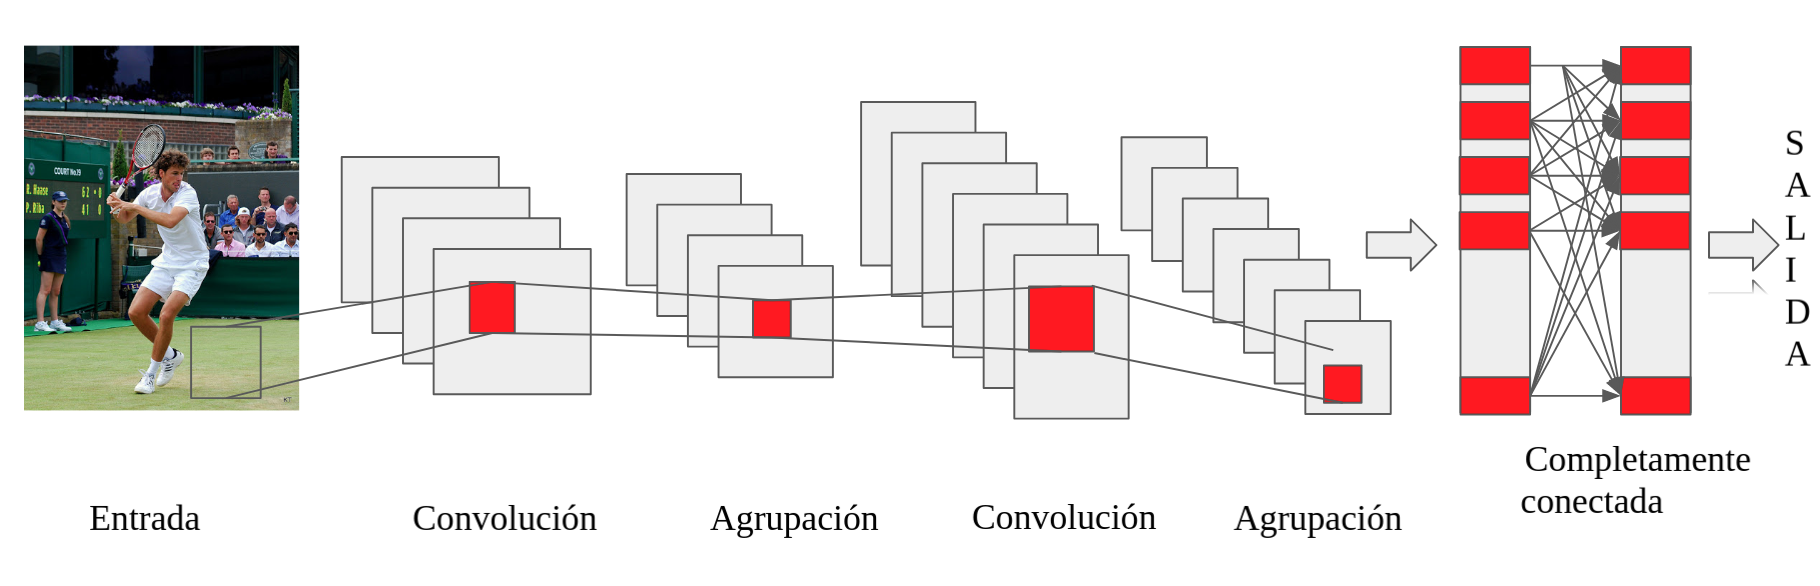
\includegraphics[width=0.9\textwidth]{img/red_cnn.png}
	\caption{Esta imagen muestra una arquitectura simplificada de una rede neuronal convolucional.}
	\label{fig:EvolucionILSVRC}
\end{figure}

\section{Word embedding}
Al igual que con las imágenes, que utilizamos las redes CNN, para obtener un vector que represente a la misma, es necesario un procedimiento para poder representar las palabras, con algún objeto matemático. Hay muchas formas de representar palabras, pero la mas conocida es word embedding, es una técnica de aprendizaje en el campo de procesamiento del lenguaje natural (PLN). Es capas de capturar el contexto de una palabra en un documento, calcular similitud semántica y sintáctica con otras palabras, etc. Word2Vec \cite{mikolov2013distributed} es una de la implementación mas conocida. Fue desarrollado por Tomas Mikolov en 2013. \\
El objetivo, es que las palabras con un contexto similar ocupen posiciones espaciales cercanas, mientras que palabras que no tienen un contexto similar estén espaciadas. Para lograr esto, se introduce cierta dependencia de una palabra de las otras palabras. Se utilizan texto para entran estos modelos, asi las palabras en el contexto de una palabra especifica, obtendrían una mayor proporción de esta dependencia.\\
En este trabajo, aprovechamos la capacidad de capturar similitudes semántica que tiene word embedding, para relacionar las clases vistas con las clases no vistas. Utilizamos un modelo pre-entrenado generado a partir de word2vec para representar las palabras de las distintas clases.

\section{Propuestas de objetos}
En problemas de detección de objetos, generalmente tenemos que encontrar todos los objetos posibles en la imagen como todos los autos todas las bicicletas, etc. La localización de objetos se refiere a identificar la ubicación de uno o varios objetos en la imagen. Un algoritmo de localización de objetos generará las coordenadas de la ubicación de los objetos con respecto a la imagen. En visión artificial, la forma más popular de representar la ubicación de los objetos es con la ayuda de cuadros delimitadores (Bounding Boxs). Existen muchos algoritmos y redes que intenta resolver este problema como por ejemplo, ventana deslizante, Edge-Boxes \cite{zitnick2014edge}, Selective search \cite{uijlings2013selective} ect. En ZSD las propuestas de objetos cumple un papel importante, ya que se necesita extraer todas las instancias de los objetos, pero también tiene que discriminar fondos como cielo, fondo de ciudad, veredas, ect. Es muy difícil encontrar un equilibrio ya que un algoritmo poco ``permisivo'' ignorara muchas instancias de objetos y por el otro extremo, se incluirá fondos y de esta manera introducir ruido en nuestro modelo. En este proyecto se usa Edge-Boxes, ya que este genera una cantidad significativamente menor a algoritmos del estilo de ventana deslizante. Aun asi, procesar todas estas propuestas es engorroso. Esto da lugar a una técnica que filtra las propuestas, denominada Supresión no máxima (NMS) \ref{fig:NMS}. Los criterios de selección de NMS se pueden elegir para llegar a resultados particulares. El criterio mas común es Intersección sobre Unión (IoU), en la imagen ~\ref{fig:IoU} se muestra como se calcula el IoU sobre dos Bounding Boxs.

\begin{figure}[H]
	\begin{subfigure}{.4\textwidth}
		\centering
		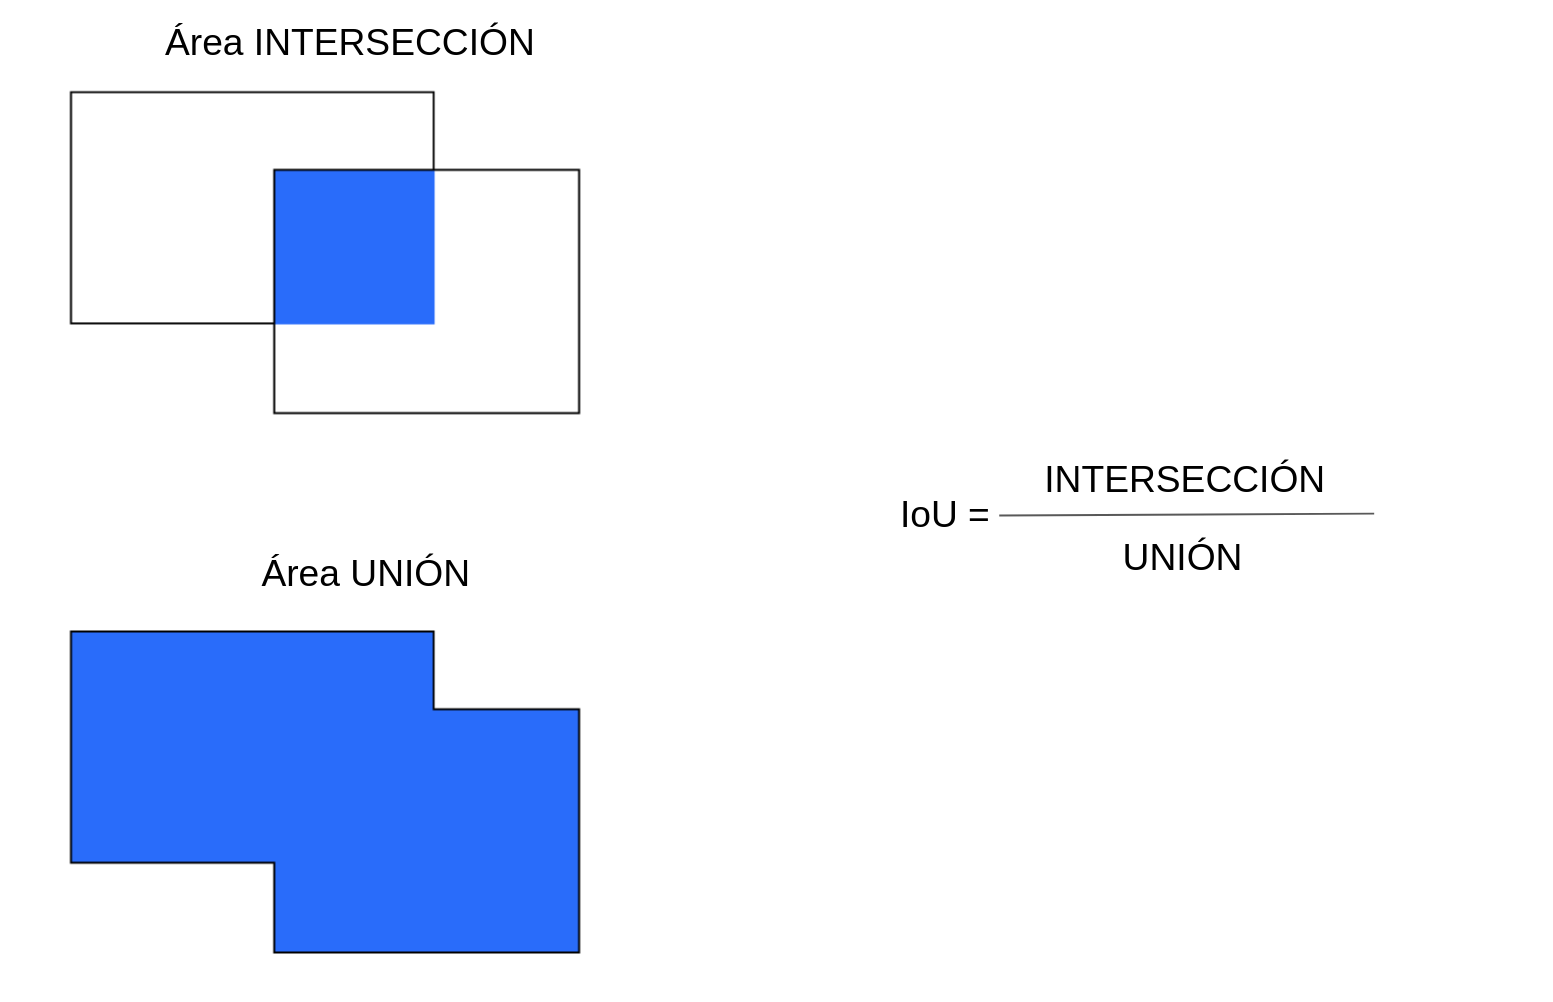
\includegraphics[width=0.7\textwidth]{img/iou.png}
		\caption{Iou}
		\label{fig:IoU}
	\end{subfigure}
	\begin{subfigure}{.6\textwidth}
		\centering
		\centering
		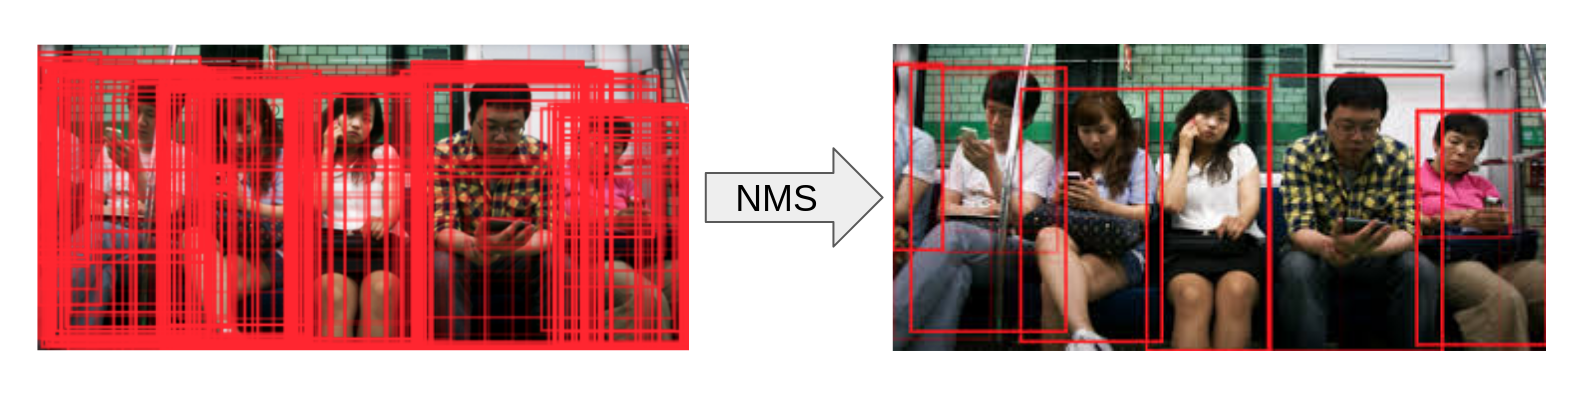
\includegraphics[width=1.1\textwidth]{img/NMS.png}
		\caption{Supresión no máxima}
		\label{fig:NMS}
	\end{subfigure}
	\caption{(a)Esta imagen muestra como se calcula el criterio Intersección sobre Unión. (b) Se muestra la salida de la propuesta de objetos y el resultado después de NMS.}
		\label{fig:RP}
\end{figure}

\section{Multimodales}

Nuestra experiencia del mundo es multimodal, vemos objetos, escuchamos sonidos, sentimos la textura, olemos los olores y probamos los sabores. La modalidad se refiere a la forma en que algo sucede o se experimenta y un problema de investigación se caracteriza como multimodal cuando incluye múltiples modalidades. Para que la inteligencia artificial avance en la comprensión del mundo que nos rodea, necesita poder interpretar y relacionar estas señales multimodales. Aunque la combinación de diferentes modalidades o tipos de información para mejorar el rendimiento parece una tarea intuitivamente atractiva, en la práctica, es un desafío combinar el nivel variable de ruido y los conflictos entre las modalidades. Además, las modalidades tienen una influencia cuantitativa diferente sobre el resultado de la predicción. La idea general es, partir de dos objetos matemáticos distintos uno de cada modal y poder transformar a ambos para lograr que pertenezcan a un tercer objeto que es la representación multimodal. Las imágenes suelen estar asociadas con etiquetas y explicaciones de texto. En este trabajo nos aprovechamos esto y tratamos de encontrar un espacio comun entre el vector que representan a la imagen del objeto y el que representa la sintaxis del mismo.
\section {Detección de objeto por disparo cero (ZSD)}
%\cite{iacobacci}
